% Options for packages loaded elsewhere
\PassOptionsToPackage{unicode}{hyperref}
\PassOptionsToPackage{hyphens}{url}
%
\documentclass[
  12pt,
]{book}
\usepackage{amsmath,amssymb}
\usepackage{lmodern}
\usepackage{ifxetex,ifluatex}
\ifnum 0\ifxetex 1\fi\ifluatex 1\fi=0 % if pdftex
  \usepackage[T1]{fontenc}
  \usepackage[utf8]{inputenc}
  \usepackage{textcomp} % provide euro and other symbols
\else % if luatex or xetex
  \usepackage{unicode-math}
  \defaultfontfeatures{Scale=MatchLowercase}
  \defaultfontfeatures[\rmfamily]{Ligatures=TeX,Scale=1}
\fi
% Use upquote if available, for straight quotes in verbatim environments
\IfFileExists{upquote.sty}{\usepackage{upquote}}{}
\IfFileExists{microtype.sty}{% use microtype if available
  \usepackage[]{microtype}
  \UseMicrotypeSet[protrusion]{basicmath} % disable protrusion for tt fonts
}{}
\makeatletter
\@ifundefined{KOMAClassName}{% if non-KOMA class
  \IfFileExists{parskip.sty}{%
    \usepackage{parskip}
  }{% else
    \setlength{\parindent}{0pt}
    \setlength{\parskip}{6pt plus 2pt minus 1pt}}
}{% if KOMA class
  \KOMAoptions{parskip=half}}
\makeatother
\usepackage{xcolor}
\IfFileExists{xurl.sty}{\usepackage{xurl}}{} % add URL line breaks if available
\IfFileExists{bookmark.sty}{\usepackage{bookmark}}{\usepackage{hyperref}}
\hypersetup{
  pdftitle={Integrated Inferences},
  pdfauthor={Macartan Humphreys and Alan M. Jacobs},
  hidelinks,
  pdfcreator={LaTeX via pandoc}}
\urlstyle{same} % disable monospaced font for URLs
\usepackage{longtable,booktabs,array}
\usepackage{calc} % for calculating minipage widths
% Correct order of tables after \paragraph or \subparagraph
\usepackage{etoolbox}
\makeatletter
\patchcmd\longtable{\par}{\if@noskipsec\mbox{}\fi\par}{}{}
\makeatother
% Allow footnotes in longtable head/foot
\IfFileExists{footnotehyper.sty}{\usepackage{footnotehyper}}{\usepackage{footnote}}
\makesavenoteenv{longtable}
\usepackage{graphicx}
\makeatletter
\def\maxwidth{\ifdim\Gin@nat@width>\linewidth\linewidth\else\Gin@nat@width\fi}
\def\maxheight{\ifdim\Gin@nat@height>\textheight\textheight\else\Gin@nat@height\fi}
\makeatother
% Scale images if necessary, so that they will not overflow the page
% margins by default, and it is still possible to overwrite the defaults
% using explicit options in \includegraphics[width, height, ...]{}
\setkeys{Gin}{width=\maxwidth,height=\maxheight,keepaspectratio}
% Set default figure placement to htbp
\makeatletter
\def\fps@figure{htbp}
\makeatother
\setlength{\emergencystretch}{3em} % prevent overfull lines
\providecommand{\tightlist}{%
  \setlength{\itemsep}{0pt}\setlength{\parskip}{0pt}}
\setcounter{secnumdepth}{5}
\usepackage{booktabs}
\usepackage{color}
\usepackage{amsmath}
\usepackage{amssymb}
\usepackage{amsfonts}

\usepackage{framed}
\setlength{\fboxsep}{.8em}

\newenvironment{blackbox}{
  \definecolor{shadecolor}{rgb}{0, 0, 0}  % black
  \color{white}
  \begin{shaded}}{\end{shaded}}

\newenvironment{headerbox}{
  \definecolor{shadecolor}{rgb}{0.8, 0.8, 0.8}  % black
  \color{black}
  \begin{shaded}}{\end{shaded}}

% \usepackage{tcolorbox}
%
% \newtcolorbox{blackbox}{
%   colback=black,
%   colframe=orange,
%   coltext=white,
%   boxsep=5pt,
%   arc=4pt}
\usepackage{amsmath}
\usepackage{color}
\usepackage{amssymb}
\usepackage{amsfonts}
\usepackage{dsfont}
\usepackage{booktabs}
\usepackage{longtable}
\usepackage{array}
\usepackage{multirow}
\usepackage{wrapfig}
\usepackage{float}
\usepackage{colortbl}
\usepackage{pdflscape}
\usepackage{tabu}
\usepackage{threeparttable}
\usepackage{threeparttablex}
\usepackage[normalem]{ulem}
\usepackage{makecell}
\usepackage{xcolor}
\ifluatex
  \usepackage{selnolig}  % disable illegal ligatures
\fi
\usepackage[]{natbib}
\bibliographystyle{apalike}

\title{Integrated Inferences}
\author{Macartan Humphreys and Alan M. Jacobs}
\date{Version: 19 November 2021}

\begin{document}
\maketitle

{
\setcounter{tocdepth}{1}
\tableofcontents
}
\hypertarget{preface}{%
\chapter*{Preface}\label{preface}}
\addcontentsline{toc}{chapter}{Preface}

This book has four main parts:

\begin{itemize}
\item
  Part I introduces causal models and a Bayesian approach to learning about them and drawing inferences from them.
\item
  Part II applies these tools to strategies that use process tracing, mixed methods, and ``model aggregation.''
\item
  Part III turns to design decisions, exploring strategies for assessing what kind of data is most useful for addressing different kinds of research questions given knowledge to date about a population or a case.
\item
  In Part IV we put models into question and outline a range of strategies one can use to justify and evaluate causal models.
\end{itemize}

We have developed an \texttt{R} package---\texttt{CausalQueries}---to accompany this book, hosted on \href{https://cran.r-project.org/web/packages/CausalQueries/index.html}{Cran}. In addition, a supplementary \href{https://macartan.github.io/causalmodels/}{Guide to Causal Models} serves as a guide to the package and provides the code behind many of the models used in this book.

\hypertarget{theory}{%
\chapter{Theories as causal models}\label{theory}}

\begin{headerbox}
We describe an approach in which theoretical claims are thought of as model justifications within a hierarchy of causal models. The approach has implications for consistency of inferences and for assessing when and how theory is useful.

\end{headerbox}

In Chapter \ref{illustratemodels}, we described a set of theories and represented them as causal models. But so far we haven't been very explicit in what we mean by a theory or how theory maps onto a causal-model framework.

In this book, we will think of theory as a type of \emph{explanation}: a theory provides an account of how or under what conditions a set of causal relationships operate. We generally express both a theory and the claims being theorized as causal models. The theory is then is a model that \emph{implies} another model---possibly with the help of some data.

To fix ideas: a simple claim might be that ``\emph{A} caused \emph{B} in case \(j\)''. This claim is itself a model, albeit a very simple one. The theory that supports this model might be of the form ``\emph{A} always causes \emph{B}'', ``\emph{A} always causes \emph{B} whenever \emph{C} (and \emph{C} holds in case \emph{j})'', or ``\emph{A} invariably causes \emph{B} and invariably \emph{B} causes \emph{C}''. These all have in common that they are arguments that could be provided to support the simple claim; in each case, if you believe the theory you believe the implication.

The rest of this short chapter builds out this idea and uses it to provide a way of characterizing when a theory is useful or not.
In the first section, we consider multiple senses in which one model might imply, and thus serve as a \emph{theory of}, another model. For one thing, we consider how one causal structure can imply (theorize) another causal structure, by including additional new nodes and nodal types that explain how or when causal effects in the original model will unfold. Next, we consider how the causal-type \emph{ranges} of models can relate to one another: one model can imply another model when the former's causal types constitute a subset of the latter's. In this situation, the theory represents a more specific, stronger claim about the kinds of causal effects that are operating. We then turn to logical relations between probabilistic models. We show how the distributions over nodal types in a simpler model structure can be underwritten by distributions over nodal types in a more detailed model structure. Here, a claim about the prevalence (or probability) of causal effects in a causal network is justified by claims about the prevalence or probability of causal effects in a more granular rendering of that network. Finally, we show how a probabilistic model plus \emph{data} can provide a theoretical underpinning for a new, stronger model.

Second, we consider how theories-as-models can be useful. In embedding theorization within the world of causal models, we ultimately have an empirical objective in mind. Theorizing a causal relationship of interest, in our framework, means elaborating our causal beliefs about the world in greater detail. As we show in later chapters, theorizing in the form of a causal model allows us to generate research designs: to identify sources of inferential leverage and to explicitly and systematically link observations of components of a causal system to the causal questions we seek to answer. In the second section of this chapter, however, we provide a high-level conceptualization of the empirical gains from theory.

In the chapter's third and final section, we show how our formalization of theory maps onto \emph{formal} theory as usually understood, showing how we can generate a causal model from a game-theoretic model.

\hypertarget{models-as-theories-of}{%
\section{\texorpdfstring{Models as \emph{theories of}}{Models as theories of}}\label{models-as-theories-of}}

Let us say that a causal model, \(M^\prime\), is a \emph{theory of} \(M\) if \(M\) is implied by \(M^\prime\). It is a theory \emph{because} it has implications. Otherwise it is a conclusion, an inference, or claim. A theory, \(M^\prime\), might itself sit atop---be supported by---another theory, \(M^{\prime\prime}\), that implies \(M^\prime\). To help fix the idea of theory as ``supporting'' or ``underlying'' the model(s) it theorizes, we refer to the theory, \(M^\prime\), as a \emph{lower}-level model relative to \(M\) and refer to \(M\) as a \emph{higher}-level model relative to its theorization, \(M^\prime\).\footnote{We note that our definition of theory differs somewhat from that given in \citet{pearl2009causality} (p207): there a theory is a (functional) causal model and a restriction over \(\times_j \mathcal{R}(U_j)\), that is, over the collection of contexts envisionable. Our definition also considers probabilistic models as theories, allowing statements such as ``the average effect of \(X\) on \(Y\) is 0.5.''}

Both structural models and probabilistic models---possibly in combination with data---imply other models. We discuss each in turn.

\hypertarget{implications-of-structural-causal-models}{%
\subsection{Implications of structural causal models}\label{implications-of-structural-causal-models}}

Structural models can imply multiple other simpler structural models. Similarly structural models can be implied by multiple more involved models.

We imagine two forms of lower level model, those that involve ``type splintering'' and those that involve ``type reduction.''

\textbf{Type splintering theorization.} Theorization often involves a refinement of causal types, implemented through the addition of nodes.
Take the very simple model, \(M\), represented in Figure \ref{fig:Highlow}(a). The model simply states that \(X\) has (or \emph{can} have) a causal effect on \(Y\).

What theories might justify \(M\)? This question can be rephrased as ``what models imply model \(M\)?'' The figure points to two possibilities. Both models \(M^\prime\) and \(M^{\prime\prime}\) imply model \(M\). They can be thought of as \emph{theories}, or lower-level model, of \(M\).

Model \(M^\prime\) differs by the addition of a node, \(K\), in the causal chain between \(X\) and \(Y\). We can say that \(M^\prime\) is a \emph{theory} of \(M\) for two reasons. First it provides a \emph{justification}---if you believe \(M^\prime\) you should believe \(M\): if \(X\) affects \(Y\) through \(K\), then \(X\) affects \(Y\). But as well as a justification it also provides an \emph{explanation} of \(M\). Suppose we already \emph{know} that \(X\) affects \(Y\) but want to know \emph{why}. If we ask, ``why does \(X\) affect \(Y\)?'', \(M^\prime\) provides an answer: \(X\) affects \(Y\) \emph{because} \(X\) affects \(K\), and \(K\) affects \(Y\).

Model \(M^{\prime\prime}\) differs by the addition of a node, \(C\), that moderates the effect of \(X\) on \(Y\). \(M^{\prime\prime}\) justifies \(M\) in the sense that if you believe \(M^{\prime\prime}\) you should believe \(M\). It provides an explanation of a kind also: if you believe model \(M^{\prime\prime}\) you likely believe that the relation between \(X\) and \(Y\) is what it is because of \(C\). Had \(C\) been different the causal relation between \(X\) and \(Y\) might have been also.

A key idea is that both \(M'\) and \(M''\) involve a redefinition of \(\theta^Y\). That is we see a change in the endogenous nodes but these in turn imply a change in the interpretation of the exogenous nodes pointing into existing endogenous nodes (such as \(Y\) in this example). We can think of part of \(\theta^Y\) being splintered off and captured by \(\theta^K\) or \(C\).

Return to models \(M\) and \(M'\) in Figure \ref{fig:Highlow}(a).
Importantly, in moving from the higher- to the lower-level model, we have effectively \emph{split} the nodal-type term \(\theta^Y\) into two parts: \(\theta^{Y_\text{lower}}\) and \(\theta^K\). Intuitively, in the higher-level model, (a), \(Y\) is a function of \(X\) and \(\theta^Y\), the latter representing all things other than \(X\) than can affect \(Y\). Or, in the language of our nodal-type setup, \(\theta^Y\) represents all of the (unspecified) sources of variation in \(X\)'s effect on \(Y\). When we insert \(K\) into the model, however, \(X\) now does not directly affect \(Y\) but only does so via \(K\). Further, we model \(X\) as acting on \(K\) in a manner conditioned by \(\theta^K\), which represents all of the (unspecified) factors determining \(X\)'s effect on \(K\). The key thing to notice here is that \(\theta^K\) now represents \emph{a portion of the variance that \(\theta^Y\) represented in the higher-level graph}: some of the variation in \(X\)'s effect on \(Y\) now arises from variation in \(X\)'s effect on \(K\), which is captured by \(\theta^K\). So, for instance, \(X\) might have no effect on \(Y\) because \(\theta^K\) takes on the value \(\theta^K_{00}\), so that \(X\) has no effect on \(K\). Put differently, any effect of \(X\) on \(Y\) must arise from an effect of \(X\) on \(K\); so \(\theta^K\)'s value must be either \(\theta^K_{01}\) or \(\theta^K_{10}\) for \(X\) to affect \(Y\). \footnote{As we emphasize further below, it is in fact only the random, unknown component of the \(X\rightarrow K\) link that makes the addition of \(K\) potentially informative as a matter of research design: if \(K\) were a deterministic function of \(X\) only, then knowledge of \(X\) would provide full knowledge of \(K\), and nothing could be learned from observing \(K\).} What \(\theta^K\) represents, then, is that part of the original \(\theta^Y\) that arose from some force other than \(X\) operating at the \emph{first} step of the causal chain from \(X\) to \(Y\).
So now, \(\theta^Y\) in the lower-level graph is not quite the same entity as it was in the higher-level graph. In the original graph, \(\theta^Y\) represented \emph{all} sources of variation in \(X\)'s effect on \(Y\). In the lower-level model, with \(K\) as mediator, \(\theta^Y\) represents only the variation in \(K\)'s effect on \(Y\). Put differently, \(\theta^Y\) has been expunged of any factors shaping the first stage of the causal process, which now reside in \(\theta^K\). We highlight this change in \(\theta^Y\)'s meaning by referring in the second model to \(\theta^{Y_\text{lower}}\).

Consider next model \(M^{\prime\prime}\) panel (c) in Figure \ref{fig:Highlow}, which also supports (implies) the higher-level model in panel \((a)\). The logical relationship between models \((a)\) and \((c)\), however, is somewhat different. Here the lower-level model \emph{specifies} one of the conditions that comprised \(\theta^Y\) in the higher-level model. In specifying a moderator, \(C\), we have extracted \(C\) from \(\theta^Y\), leaving \(\theta^{Y_\text{lower}}\) to represent all factors \emph{other than \(C\)} that condition \(Y\)'s response to its parents. More precisely, \(\theta^{Y_\text{lower}}\) now represents the set of nodal types defining how \(Y\) responds jointly to \(X\) and \(C\). Again, the relabeling as \(\theta^{Y_\text{lower}}\) reflects this change in the term's meaning. Whereas in Model \(M^{\prime}\) we have extracted \(\theta^K\) from \(\theta^Y\), in Model \(M^{\prime\prime}\), it is \(C\) itself that we have extracted from \(\theta^Y\), substantively specifying what had been just a random disturbance.

\begin{figure}

{\centering 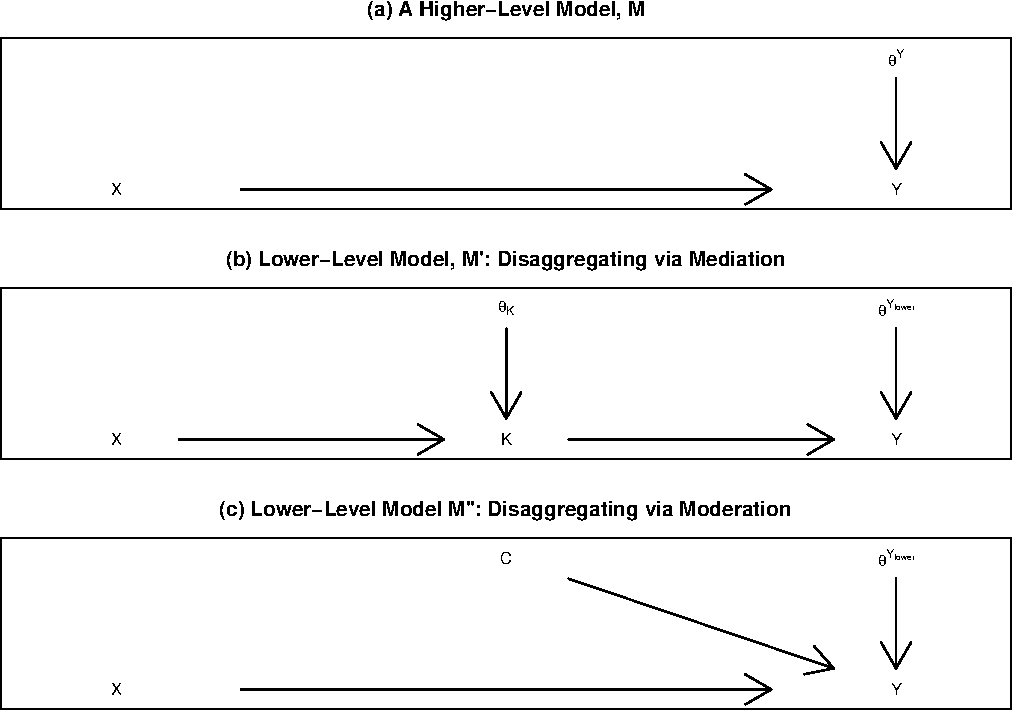
\includegraphics[width=0.8\linewidth]{ii_files/figure-latex/Highlow-1} 

}

\caption{Here we represent the simple claim that one variable causes another, and two theories --- lower-level models --- that could explain this claim. Both model (b) and model (c) involve theorization via disaggregation of nodes.}\label{fig:Highlow}
\end{figure}

\textbf{Type-reducing theorization.} There is a second way in which we might imagine a model being implied by another model that does not involve a change in nodes. Let \(\Theta(\mathcal M_1)\) denote the set of causal types in model \(\mathcal M_1\). Then we can say that \(\mathcal M_0\) implies \(\mathcal M_1\) if \(\Theta(\mathcal M_0)\subseteq \Theta(\mathcal M_1)\). Informally this means that any relation admitted by theory \(\mathcal M_0\) is representable in model \(\mathcal M_1\), though the converse may not be true. We can think of a theory of \(\mathcal M_1\) as a \emph{restriction} of ranges of \(\Theta(M_1)\).

We illustrate the idea in Figure \ref{fig:Highlowreduce}. In panel (a) of the figure, we have a model, \(\mathcal M_1\) in which \(Z\) can have both a direct and an indirect effect (via \(X\)) on \(Y\). Suppose that we believed that \(\mathcal M_1\) was technically true but overly permissive, in the sense that it allowed for causal relations that we do not in fact believe are operating. We might believe, for instance, that \(Z\) has no direct effect on \(Y\) and that \(Z\) has no negative effects on \(X\) --- the beliefs we would need to hold to treat \(Z\) as an instrument for \(X\). We could thus write down a lower-level model, \(\mathcal M_0\),in which we have \emph{reduced} the type space accordingly. Specifically, in \(\mathcal M_0\), we would restrict the nodal types at \(Y\) to only the \(\theta^Y_{0000}\), \(\theta^Y_{1100}\), \(\theta^Y_{0011}\), and \(\theta^Y_{1111}\); and we would reduce the nodal types at \(X\) to \(\theta^X_{00}\), \(\theta^X_{01}\), and \(\theta^X_{11}\). In panel (b), we (somewhat loosely) represent \(\mathcal M_0\). We have now eliminated the arrow from \(Z\) to \(Y\) to represent the dropping of all nodal types involving a direct effect of \(Z\) on \(Y\); not pictured is the montonicity assumption at \(X\). However, we have relabeled the nodal-type nodes for both \(X\) and \(Y\) to represent the fact that these are different objects from the nodal type nodes in the higher-level model.\footnote{We drop the arrow in Figure \ref{fig:Highlowreduce}, however, in order to help visually convey the difference between the two models. In fact, we would construct \(\mathcal M_0\) by placing restrictions at nodes in \(\mathcal M_1\), rather than by changing the model's structure, so that the allowed types in \(\mathcal M_0\) form a subset of those in \(\mathcal M_1\).}

Thus, while we can theorize by adding substantive nodes to a model and thus splitting types, we can also theorize by maintaining existing nodes but constraining relations among them. In both forms of theorization, we start with a model that allows for a broad, and possibly unknown, range of possibilities: for instance, a broad range of paths through which or conditions under which \(X\) might affect \(Y\) or a broad range of causal effects operating at each node. Theorization of both forms then involves making a \emph{stronger} claim: for instance, a claim about \emph{how} or \emph{when} \(X\) affects \(Y\) (via type-splintering) or a claim about the \emph{particular} causal effects operating at a given node (via type-reduction). In both forms of theory, believing the stronger claim in the lower-level model implies believing the weaker claim in the higher-level model. Further, both modes of theorization also map nicely onto common ways in which we think about theory-development in the social sciences: we theorize mechanisms, sources of heterogeneity, and directions of effects (starting with a belief that \(X\) affects \(Y\), for instance, and moving to a more constrained belief about whether that effect is positive or negative).

Finally, as we speak to below, theorization of both forms can generate gains for causal inference, by allowing us to use data in ways that we are unable to use it in the higher-level model.

\textbf{Preserving (conditional) independencies}

Not all potential mappings from higher- to lower-levels are permitted. In particular, when theorizing, we may \emph{add} but may not \emph{remove} independencies implied by the original model. If two variables are independent--- or conditionally independent given a third variable---in one model, then this same relation of independence (or conditional independence) must be captured in any theory of that model. For instance, if we start with a model of the form \(X \rightarrow Y \leftarrow W\), where \(W\) and \(X\) are independent, we could not theorize this model by adding an arrow from \(X\) to \(W\). A theory can have \emph{additional} conditional independencies not present in the higher-level model, as in the example in Figure \ref{fig:Highlowreduce}. But we may not theorize \emph{away} (conditional) independencies insisted on by our higher-level claim.

This is a key part of what it means for the lower-level model to \emph{justify} the higher-level model. A model makes claims about what is (conditionally) independent of what. The claims about conditional independence implied by the higher-level model must therefore be warranted by (conditional) independencies operating in the lower-level model. If we introduce new dependencies via theorization, then our higher-level model (which excludes these dependencies) would no longer be justified by the lower-level model.

\begin{figure}

{\centering 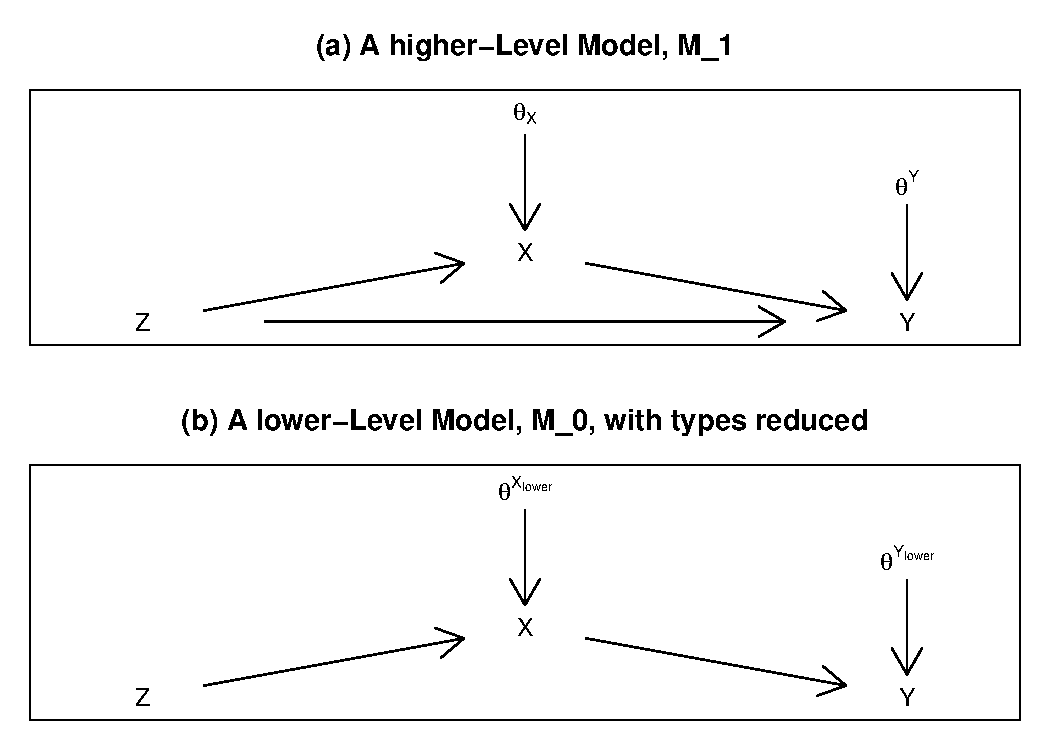
\includegraphics[width=0.8\linewidth]{ii_files/figure-latex/Highlowreduce-1} 

}

\caption{Here we represent theorization via type-reduction. Though we show the removal of an arrow to help convey the idea, we would in fact reduce types by imposing restrictions on the nodal types at Y within the same DAG.}\label{fig:Highlowreduce}
\end{figure}

\hypertarget{probabilistic-causal-models}{%
\subsection{Probabilistic causal models}\label{probabilistic-causal-models}}

At the structural level, then, there are two types of theory, or two types of relations between levels of model: those defined by type-splintering and those defined by type-reduction. In general, we will want to be working with probabilistic causal models --- i.e., those that include distributions over nodal types. We can describe straightforwardly how distributions in a higher-level model relate to --- and must change with --- distributions at the lower level. Indeed, it is these relations that unlock the opportunity for reaping empirical gains from theory.

\textbf{Theoretical implications of probabilistic models.} Suppose we start with the mediation model in panel (b) of Figure \ref{fig:Highlow}. Wen then add to it a distribution over \(\theta^K\) and \(\theta^Y_{lower}\), giving us a probabilistic causal model that we will denote \(\mathcal M^p_{lower}\). \(\mathcal M^p_{lower}\), in turn, implies a higher-level probabilistic model, \(\mathcal M^p_{higher}\), formed from the structure of Model (a) in Figure \ref{fig:Highlow}, and a \emph{particular} distribution over \(\theta^Y\): specifically, \(\theta^Y\) will have the distribution that preserves the causal relations implied by the beliefs in \(\mathcal M^p_{lower}\). Thus, for instance, the probability that \(X\) has a positive effect on \(Y\) in \(\mathcal M^p_{higher}\) is \(\theta^{Y}_{01}\); the probability that \(X\) has a positive effect on \(Y\) in \(\mathcal M^p_{lower}\) is \(\theta^{K_{lower}}_{01}\theta^{Y_{lower}}_{01} + \theta^{K_{lower}}_{10}\theta^{Y_{lower}}_{10}\). Consistency then requires that \(\theta^{M_{lower}}_{01}\theta^{Y_{lower}}_{01} + \theta^{K_{lower}}_{10}\theta^{Y_{lower}}_{10} = \theta^{Y_{higher}}_{01}\). So the value of \(\theta^{Y_{higher}}_{01}\) is \emph{implied} by \(\theta^{K_{lower}}_{01},\theta^{Y_{lower}}_{01}, \theta^{K_{lower}}_{10},\theta^{Y_{lower}}_{10}\), but not vice-versa.

\textbf{Deducing models from theory and data.} Now we can see what happens if we bring data to the lower-level model. A probabilistic causal model coupled with data implies another probabilistic causal model via Bayes rule. For this reason, we can fruitfully think of an initial model as being a \emph{theory of} an updated model, coupled with data. Thought of in this way we have clarity over what is meant when we turn to theory to support a claim, but also what is meant when we seek to justify a theory. We might imagine a scholar arguing: ``\(\mathcal M_1\): \(X\) caused \(Y\) in country \(j\).'' When pushed for a justification for the claim they provide the lower level model: ``\(\mathcal M_0:\) the average effect of \(X\) on \(Y\) in countries with feature \(C=1\) is 0.95, making it likely that \(X\) caused \(Y\) in this case.'' Here \(\mathcal M_1\) is implied by \(\mathcal M_0\) coupled with data \(C=1\). If pushed further as to why that theory is itself credible they might point to a lower level model consisting of structural model \(X\rightarrow Y \leftarrow C\) plus flat priors coupled with data on \(X,Y\) and \(C\). At each stage, as more justification is provided, the researcher formally provides lower-level models.

Moving up, as more data is provided, more ``specific'' higher level models emerge, justified by lower models plus data. These models are more specific in the sense that they are implied by the higher level models, plus data, but not vice versa. But they are also (generally) more specific in a second sense: that they make stronger statements about how causal processes operate.\footnote{This is not universally true, a point we return to below.} They place greater weight on a smaller set of causal claims.\footnote{In frequentist frameworks we often think of analysis as implementing up-or-down empirical tests against data to parse between theories that should be maintained and theories that should be rejected. In a Bayesian framework we think more continuously of shifting our beliefs across causal possibilities within a multi-dimensional theoretical space.}

As the simplest illustration, we might imagine beginning with an \(X\rightarrow Y\) model, \(\mathcal M_1\), in which, \(X\) and \(Y\) are binary, and we we believe that \(Y\) possibly responds to \(X\). If we have ``flat'' priors over causal types, in the sense described in Chapter \ref{bayeschapter}, then our prior uncertainty over the proposition that \(X\) causes \(Y\), under this model, is large; as is our uncertainty that \(Y=1\) is due to \(X=1\) in a given case. In other words, given our theory, we are uncertain about the proposition \(\mathcal M_3\): \(X\) caused \(Y\). However, if we then receive a lot of data, \(\mathcal D\), showing strong relations between \(X\) and \(Y\), then our updated model \(\mathcal M_2\), formed from combining \(\mathcal D\) and \(\mathcal M_1\) allows us to infer that \(X\) caused \(Y\) in this case with greater certainty.

Thus our new theory \(\mathcal M_2\) is (a) formally similar to \(\mathcal M_1\), (b) formed as a product of past theory plus evidence, here justified by \(\mathcal M_1\) given data \(\mathcal D\), and (c) capable of providing sharper implications than past theory.\footnote{As a general matter an updated theory may not provider sharper claims for all queries. That is, in practice, posterior variance over queries can increase with more data. As a simple illustration: say, we start out thinking that the probability that an outcome is due to conditions A, B, or C is .9, .05, and .05, respectively. If I find evidence that convinces me that A is not the cause, then I shift (a) to greater certainty about whether A was the cause but (b) greater uncertainty about whether B was the cause.}

In this way, Bayesian updating provides a simple and coherent way of thinking about the integration of theory and data.

\hypertarget{theorygains}{%
\section{Gains from theory}\label{theorygains}}

We now turn to consider how to think about whether a theory is \emph{useful}. We are comfortable with the idea that theories, or models more generally, are wrong. Models are not full and faithful reflections of reality; they are maps designed for a particular purpose. We make use of them because we think that they \emph{help} in some way.

But how do they actually help, and can we quantify the gains we get from using them?

We think we can. Using the notion of hierarchies of models, imagine we begin with model \(\mathcal M_1\), which together with data \(\mathcal D\), implies claim \(\mathcal M_2\). We then posit theory \(\mathcal M_0\) of \(\mathcal M_1\), so \(\mathcal M_0\) implies \(\mathcal M_1\). But when we bring \(\mathcal D\) to \(\mathcal M_0\) we get a new model, \(\mathcal M_2'\), that is different---and, hopefully, better---than \(\mathcal M_2\). Our gain from theory \(\mathcal M_0\) should be some summary of how much better \(\mathcal M_2'\) is than \(\mathcal M_2\).

Here is an illustration using a theory that allows use of the ``front-door criterion.''

Imagine that we have data on three variables, \(X\), \(Y\), and \(K\). We begin, however, with a model \(\mathcal M_1\) with confounding: \(C \rightarrow X \rightarrow Y \leftarrow C\). \(\mathcal M_1\) includes nodes for two of the three variables we have data on, \(X\) and \(Y\), but not \(K\). Assume, further, that we do not have data on node \(C\), the confound.

Suppose that we observe a strong correlation between \(X\) and \(Y\) and infer \(\mathcal M_2\): that \(X\) is a likely cause \(Y\). Our inference under \(\mathcal M_2\) is, however, quite uncertain because we are aware that the correlation may be due to the confound \(C\).

Suppose now that we posit the lower-level model \(\mathcal M_0\): \(C \rightarrow X \rightarrow K \rightarrow Y \leftarrow C\). \(\mathcal M_0\) now lets us make better use of data \(K\). If we observe, for instance, that \(X\) and \(K\) are uncorrelated, then we infer with confidence that in fact \(X\) did not cause \(Y\), despite the correlation.

Thus, in return for specifying a theory of \(\mathcal M_1\), we have been able to make better use of data and form a more confident conclusion. In this case, stating the theory, \(\mathcal M_0\), does not alter our \emph{priors} over our query. Our prior over the effect of \(X\) on \(Y\) may be identical under \(\mathcal M_1\) and \(\mathcal M_0\)---but our conclusions, given data, differ because the theory lets us make use of the data on \(K\), which we could not do under \(\mathcal M_1\) (which did not include \(K\)).

In other situations, we might imagine invoking a theory that does not necessarily involve new data but that allows us to make different, perhaps tighter inferences using the same data. An example might be the invocation of a type-reducing theory that involves a monotonicity restriction or exclusion restriction that allows for identification of a quantity that would not be identifiable without the theory.

Thus, one reason to theorize our models --- develop lower-level models that make stronger claims --- is to be able to reap greater inferential leverage from the more elaborate theory.

But are we, in fact, better off?

We might imagine answering the question in different ways: from an internal or external position, and from an \emph{ex ante} or \emph{ex post} perspective.

In all cases we ask how much better do we do as a result of making use of a theory.

If we are willing to posit an external ground truth, then we can define ``better'' in objective terms. An \emph{ex post}, objective way of operationalizing ``better'' is to assess the size of the error we make relative to the ground truth, from an inference that uses a theory, compared to an inference that does not make use of the theory. An objective \emph{ex ante} approach might be to ask what the expected error is from conclusions one draws given a theory. For instance: how wrong are we likely to be if we base our best guess on our posterior mean? ``How wrong'' might be operationalized in terms of mean squared error---the square of the distance between the truth and the posterior mean.\footnote{Other loss functions could be used, including functions that take account of the costs of collecting additional data or to the risks associated with false diagnoses. For instance, in \citet{heckerman1991toward}, an objective function is generated using expected utility gains from diagnoses generated based on new information over diagnoses based on what is believed already. In their treatment \citep[Equation 6]{heckerman1991toward}, the expected value of new information \(K\), given existing information \(W\) is: \(\sum{K}P(K|W)( EU(d(Q,W,K)|W, K) - EU(d(Q, W)|W, K))\) where \(EU\) is expected utility and \(d\) is the optimal inference (diagnosis) given available data. Note that the diagnosis can take account of \(K\) when it is observed, but the expected utility depends on \(K\) whether or not it is observed, as \(K\) carries information about the state of interest.}

A more subjective approach would be to ask about the reductions in posterior variance. \emph{Ex post} we can define ``better'' as the reduction in posterior variance from conclusions that make use of a theory compared to conclusions that do not. We might also think about the \emph{expected posterior variance}: how certain do you expect you will be after you make use of this new information?

More formally, imagine a situation in which there is an unknown parameter \(q\) and we have a data strategy that produces a distribution over data \(k\), given \(q\). Let \(p(q,k)\) denote the joint prior distribution over \(q\) and \(k\) with marginal distributions \(p(k)\) and \(p(q)\). For any \(k\) there is posterior estimate \(q_k\).

The squared error, given \(k\) is just \((q - q_k)^2\).

The \emph{expected} squared error is:

\[ESE := \int_q\int_k \left({q}_k-q\right)^2p(k, q)dkdq \]

This takes the error one might get with respect to any true value of the parameter (\(q\)), given the data one might see given \(q\) and the inferences one might draw.

For any \(k\) we might write the posterior variance as \(v_k\).

The \emph{expected} posterior variance can be written:

\[EV := \int_k v_k p(k)dk\]

This takes the posterior variance, given some data, over all the possible data one might see given marginal distribution \(p(k)\).

Interestingly, if we assess expectations using the same priors as you use for for forming posteriors the expected posterior variance and expected squared error are equivalent \citep{scharf1991statistical}.
To see this, we take advantage of the fact that \(p(q,k) = p(k)p(q|k) = p(q)p(k|q)\) and that \(p(q|k)\) gives the posterior distribution of \(q\) given \(k\). We then have:

\begin{align}
ESE &= \int_q\int_k \left({q}_k-q\right)^2p(q,k)dkdq \\
    &= \int_k\int_q \left({q}_k-q\right)^2p(k)p(q|k)dq dk \\
    &= \int_k\left[\int_q \left({q}_k-q\right)^2p(q|k)dq\right]p(k)dk \\
    &= \int_k v_k p(k)dk  = EV
\end{align}

Note that the key move is in recognizing that \(p(q |k)\) is in fact the posterior distribution on \(q\) given \(k\). In using this we assume that the same distribution is used for assessing error and for conducing analysis---that is we take the researcher's prior to be the relevant one for assessing error.

Moreover, it is easy to see that whenever inferences are sensitive to \(K\), the \emph{expected} variance of the posterior will be lower than the variance of the prior. This can be seen from the law of total variance, written here to highlight the gains from observation of \(K\), given what is already known from observation of \(W\).\footnote{See \citet{raiffa1961applied}. A similar expression can be given for the expected posterior variance from learning \(K\) in addition to \(W\) when \(W\) is not yet known. See, for example, Proposition 3 in \citet{geweke2014analysis}.}\\
\[Var(Q|W) = E_{K|W}(Var(Q|K,W)) +Var_{K|W}(E(Q|K,W))\]

However, although \emph{expected} posterior variance goes down, it is still always possible that posterior variance rises. The increase in uncertainty does not, however, mean you haven't been learning. Rather, you have learned that things aren't as simple as you thought.

One way to capture this idea that, although we are more uncertain, we think we are better off now than we were, is to ask: how much better are our guesses having observed \(K\) compared to what we would have guessed before, \emph{given} what we know having observed \(K\)? We will call this ``Wisdom'' to reflect the idea that it values appreciation of justifiable uncertainty:

\[Wisdom  = \int(q_0 - q)^2 - (q_k - q)^2 p(q | k)dq\]

This metric captures how much better off we are with the guess we have made given current data (\(q_k\)) compared to the guess we would have made if we had a theory that did not let us make use of it (\(q_0\)), knowing what we know having observe \(K\) (\(p(q|k)\).

An advantage of this conceptualization is that we can still record gains in learning even if the learning operates such that the posterior variance is larger than the prior variance. Even so, the implications for strategy are the same since wisdom is maximized by a strategy that reduces expected squared error.

Thus expected wisdom, is:

\begin{align}
\text{Expected Wisdom}  &= \int_q(q_0 - q)^2dq - \int_k\int_q(q_k - q)^2 p(q, k)dqdk \\
&= \text{Prior variance} - \text{Expected Posterior Variance}
\end{align}

We close with a reminder. Although expected reduction in variance and expected wisdom are both positive, both are are fundamentally subjective ideas, that presuppose the theory is correct. In contrast the expected error measure can be assessed under rival theoretical propositions and so allow for the real possibility that the gains of invoking a theory are negative.

\hypertarget{formal-theories-and-causal-models}{%
\section{Formal theories and causal models}\label{formal-theories-and-causal-models}}

It is relatively easy to see how the ideas above play out for what might be called empirical models. But in social sciences ``theory'' is a term sometimes reserved for what might be called analytic models. In this last section we work through how to use this framework when seeking to bring analytic models to data.

Let's start with analytic models. As an example we might consider the existence of ``Nash equilibria.'' Nash considered a class of settings (``normal form games'') in which each player \(i\) can choose an action \(\sigma_i\) from set \(\Sigma_i\) and receives a payoff \(u_i\) that depends on the actions of all players. A particular game, \(\Gamma\) is the collection of players, action sets, and payoffs.

Nash's theorem relates to the existence of a collection of strategies with the property that each strategy would produce the greatest utility for each player given the strategies of the other players. Such a collection of strategies is called a Nash equilibrium.

The claim that such a collection of strategies exists in these settings is an analytic claim. Unless there are errors in the derivation of the result, the claim is true in the sense that the conclusions follow from the assumptions. There is no evidence that we could go looking for in the world to assess the claim. The same can be said of the theoretical claims of many formal models in social sciences; they are theoretical conclusions of the if-then variety \citep{clarke2012model}.

We will refer to theories of this form as ``analytic theories.''

When researchers refer to a theory of populism or a theory of democratization however they generally do not have such pure theories in mind. Rather they have in mind what might be called ``applied theories'' (or perhaps more simply ``scientific theories'' or ``empirical theories''): general claims about the relations between objects in the world. The distinction here corresponds to the distinction in \citet{peressini1999applying} between ``pure mathematical theories'' and ``mathematized scientific theories.''\footnote{Or see the distinction, for instance in in Keynes, between pure theory and applied theory.}

Applied theory, in this sense, is a collection of claims with \emph{empirical} content: an applied theory refers to a set of propositions of causal relations in the world that might or might not hold, and is susceptible to assessment using data. These theories might look formally a lot \emph{like} analytic theories but it is better to think of them as translations at most. The relations between nodes of an applied theory are a matter of conjecture not a matter of necessity.\footnote{\citet{peressini1999applying} distinguishes between ``applied mathematical theories'' and ``mathematized scientific theories'' on the grounds that not all mathematized theories are an application of a pure theory.}

Though it is not standard practice, formal models produced by game theorists can often be translated and then represented using the notation of structural causal models in this way. Moreover, doing so may be fruitful. Using the approach described above we can then assess the utility of the applied theory, if not the pure theory itself.

For two players, for instance, we might imagine a representation of a game as shown in Figure \ref{fig:nfg}.

\begin{figure}

{\centering 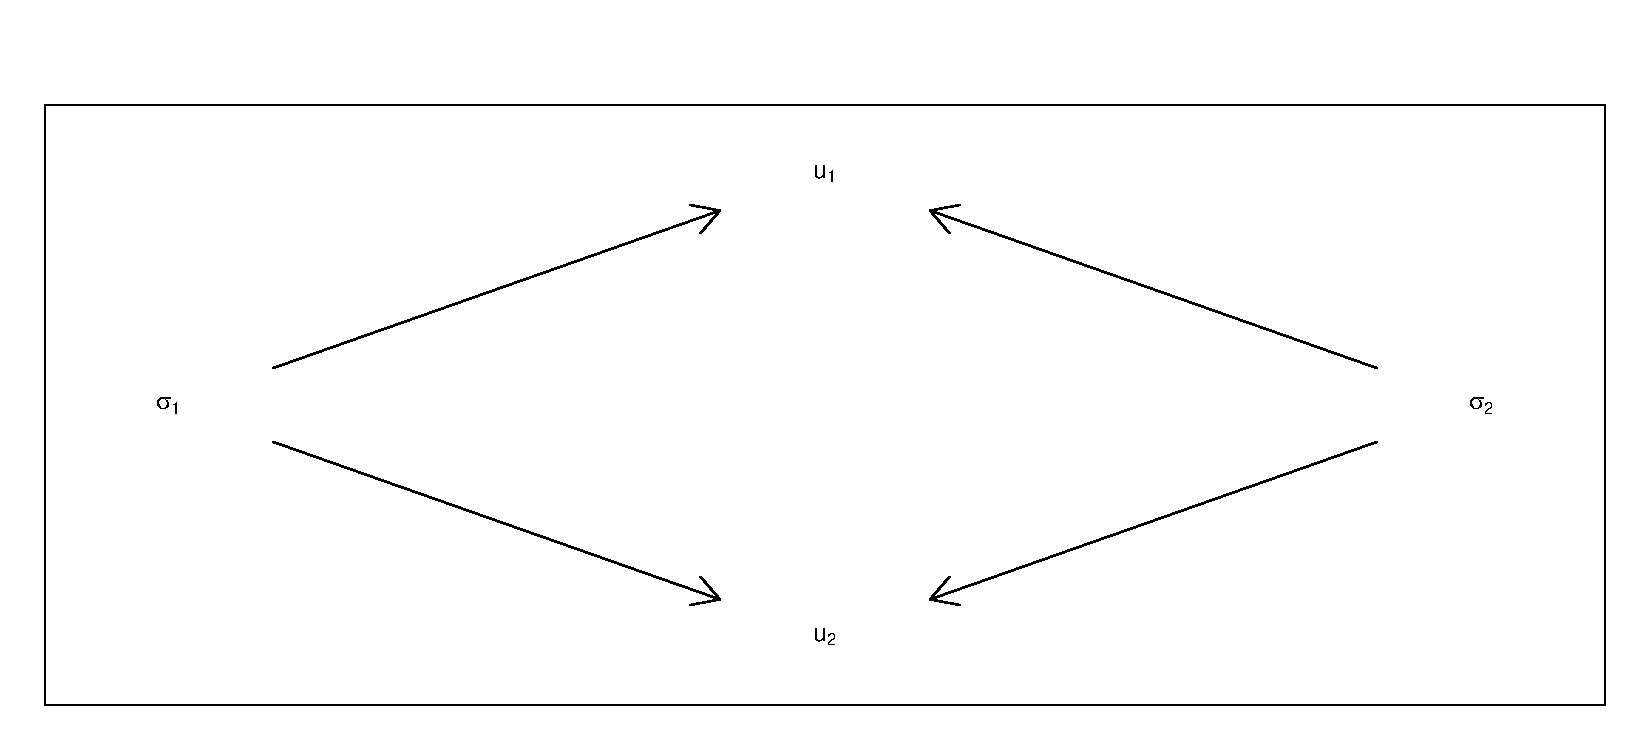
\includegraphics[width=0.8\linewidth]{ii_files/figure-latex/nfg-1} 

}

\caption{Formal structure of a normal form game.}\label{fig:nfg}
\end{figure}

Here the only functional equations are the utility functions. The utilities, given actions, are the implications of the theory, and so this is just a theory of how outcomes depend on social actions. It is not---yet---a behavioral theory.

In contrast to Nash's theorem regarding the existence of equilibria, a behavioral theory might claim that in problems that can be represented as normal form games, players indeed play Nash equilibrium. This is a theory about how people act in the world. We might call it Nash's theory.

How might this theory be represented as a causal model? Figure \ref{fig:nfg2} provides one representation.

\begin{figure}

{\centering 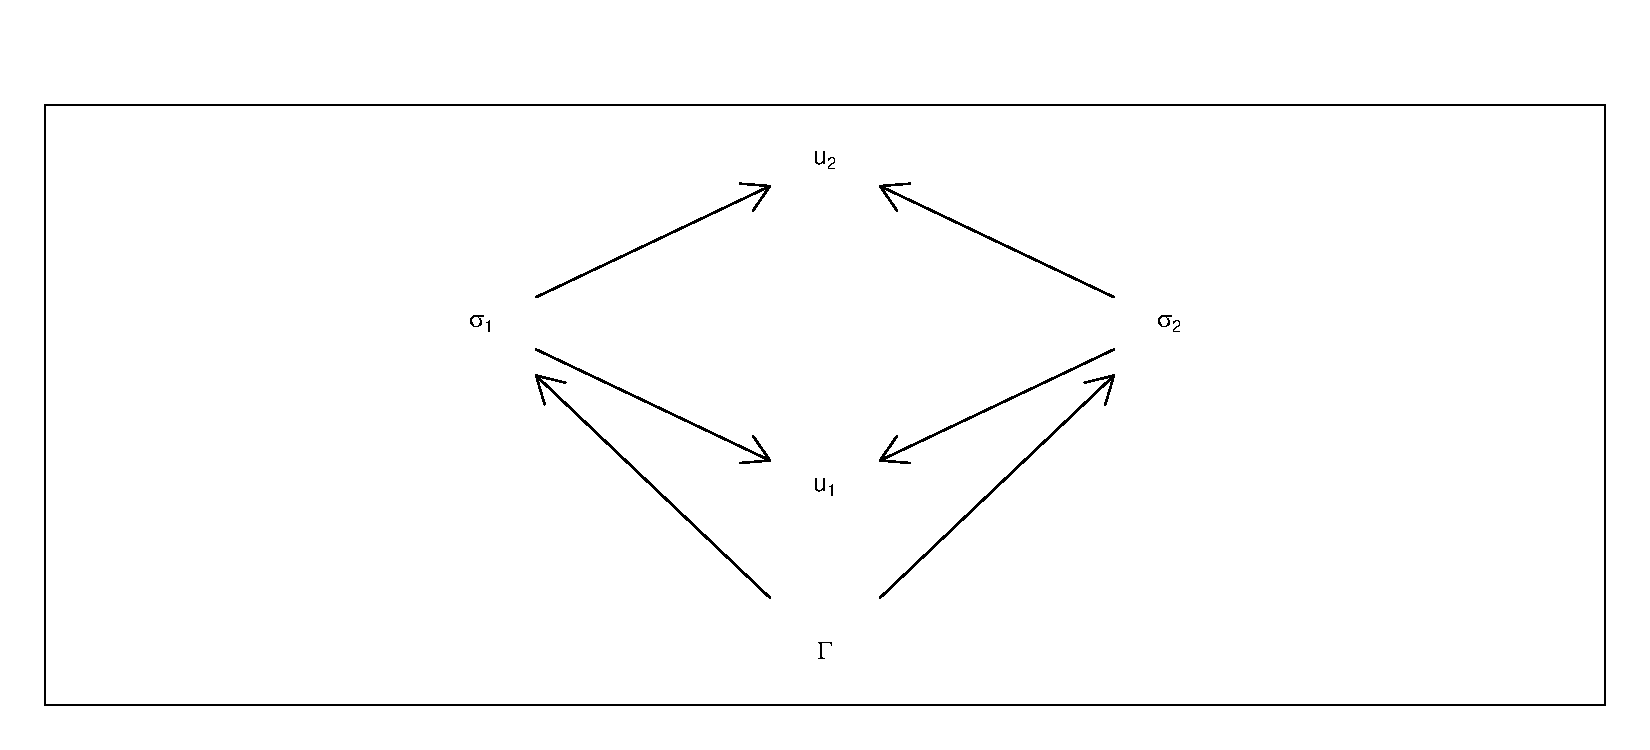
\includegraphics[width=0.8\linewidth]{ii_files/figure-latex/nfg2-1} 

}

\caption{Formal structure of a normal form game.}\label{fig:nfg2}
\end{figure}

Here beliefs about the game form (\(\Gamma\)) results in strategy choices by actors. If players play according to Nash's theory, \emph{the functional equations for the strategy choices are given by the Nash equilibrium solution itself}, with a refinement in case of multiplicity.

This model represents what we expect to happen in a game under Nash's theory and we can indeed see if the relations between nodes in the world look like what we expect under the theory. But it does not provide much of an \emph{explanation} for behavior.

A lower level causal model might help. In Figure \ref{fig:nfg3}
the game form \(\Gamma\) determines the beliefs about what actions the other player would make (thus \(\sigma_2^e\) is 1's belief about 2's actions). The functional equations for \(\sigma_2^e\) and \(\sigma_1^e\) might, for instance, be the Nash equilibrium solution itself: that is, players expect other players to play according to the Nash equilibrium (or in the case of multiple, a particular equilibrium selected using some refinement). The beliefs in turn, together with the game form (which contains \(u1, u_2\)), are what cause the players to select a particular action. The functional equation for \(\sigma_1\) might thus be \(\sigma_1 = \arg \max_\sigma u_1(\sigma, \sigma_2^e)\).

\begin{figure}

{\centering 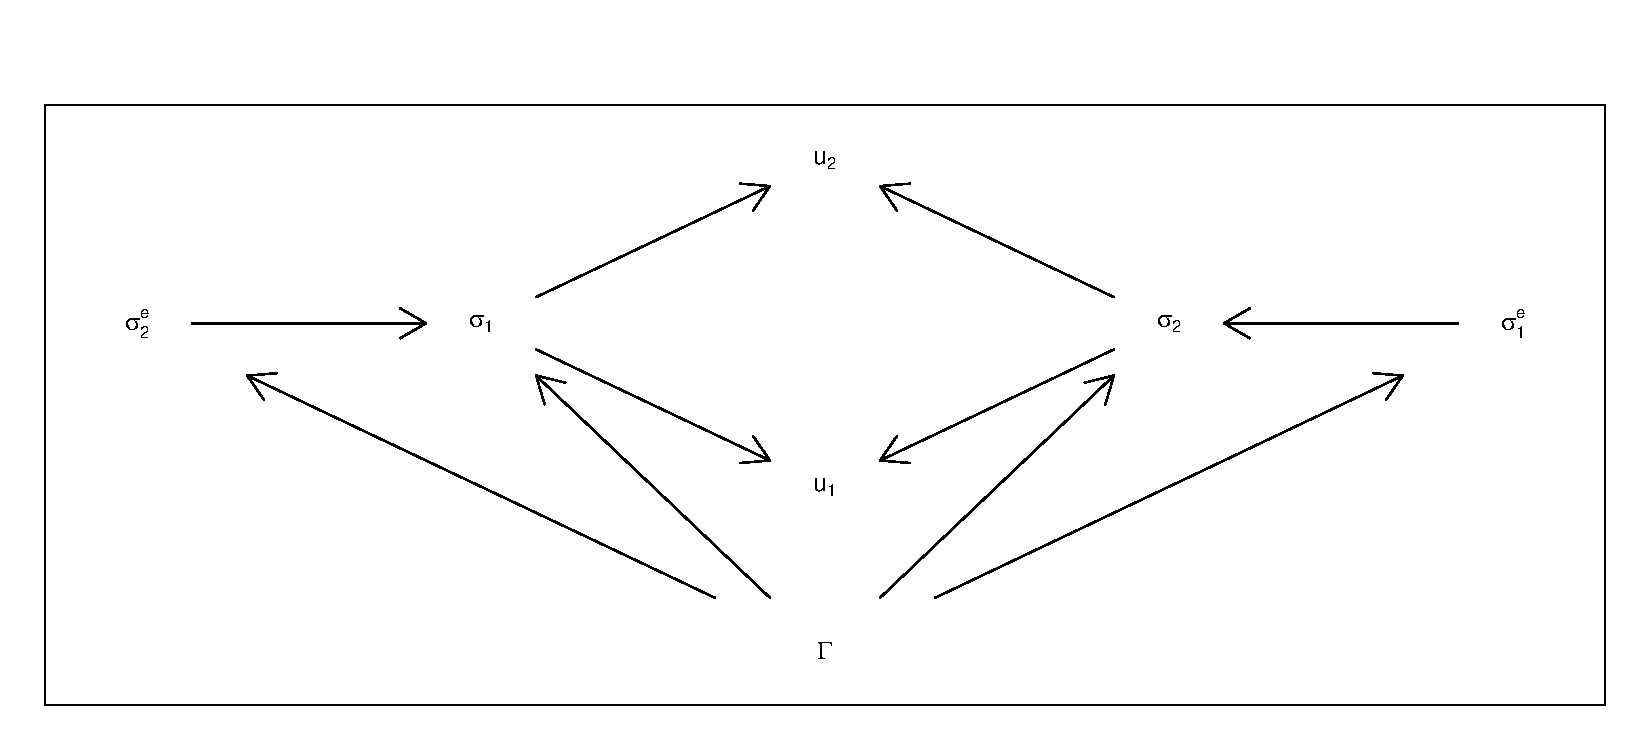
\includegraphics[width=0.8\linewidth]{ii_files/figure-latex/nfg3-1} 

}

\caption{Formal structure of a normal form game.}\label{fig:nfg3}
\end{figure}

This representation implies a set of relations that can be compared against empirical patterns. Do players indeed hold these beliefs when playing a given game? are actions indeed consistent with beliefs in ways specified by the theory. It provides a theory of beliefs and a theory of individual behavior as well as an explanation for social outcomes.

The model in Figure \ref{fig:nfg3} provides a foundation of sorts for Nash's theory. It suggests that players play Nash equilibria \emph{because} they expect others to and they are utility maximizers. But this is not the only explanation that can be provided; alternatively behavior might line up with the theory without passing through beliefs at all as suggested in some accounts from evolutionary game theory that show how processes might select for behavior that corresponds to Nash even if agents are unaware of the game they are playing.

One might step still further back and ask \emph{why} would actors form these beliefs, or take these actions, and answer in terms of assumptions about actor rationality. Figure \ref{fig:nfg4} for instance is a model in which actor rationality might vary and might influence beliefs about the actions of others as well as reactions to those beliefs. Fully specified functional equations might specify not only how actors act when rational but also how they react when they are not. In this sense the model in Figure \ref{fig:nfg4} both nests Nash's theory and provides an explanation for why actors conform to the predictions of the theory.

\begin{figure}

{\centering 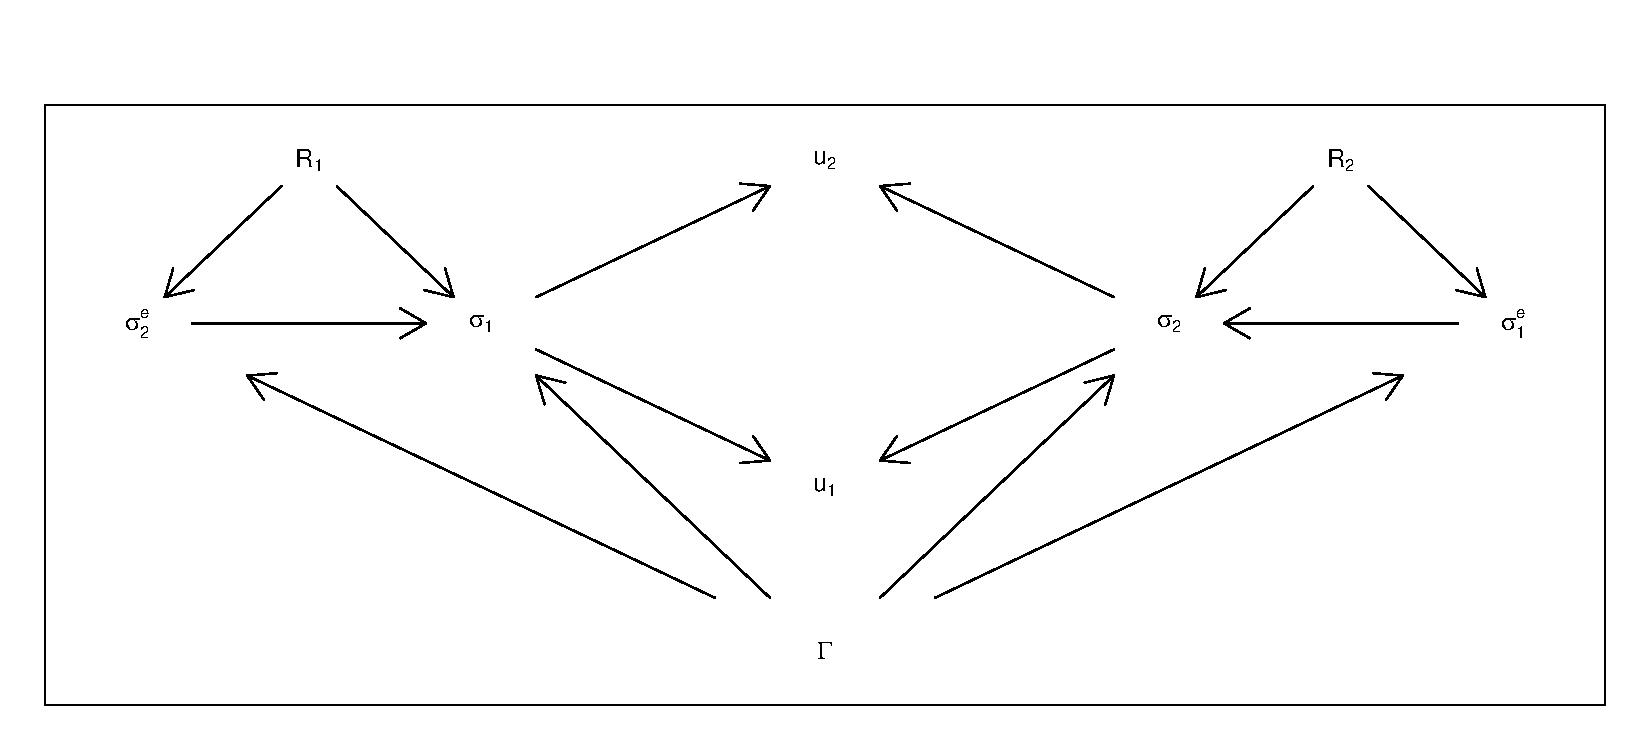
\includegraphics[width=0.8\linewidth]{ii_files/figure-latex/nfg4-1} 

}

\caption{Formal structure of a normal form game.}\label{fig:nfg4}
\end{figure}

In a final elaboration we can represent a kind of underspecification of Nash's theory that make it difficult to take the theory to data. In the above we assumed that players chose actions based on expectations that the other player would play the Nash equilibrium---or that the theory would specify which equilibrium in the case of multiplicity. But it is well known that Nash's theory often does not provide a unique solution. This indeterminacy can be captured in the Causal model as shown in Figure \ref{fig:nfg5} where a common shock---labelled \(\nu\), and interpreted as norms---interacts with the game form to determine the expectations of other players.

The functional equation for expectations can then allow for the possibility that (i) there is a unique equilibrium invariably chosen and played by both (ii) or a guarantee that players are playing one or other equilibrium together but uncertainty over which one is played, or (iii) the possibility that players are in fact out of sync, with each playing optimal strategies given beliefs but nevertheless not playing the same equilbria.

Nash's theory likely corresponds to position (ii). It can be captured by functional equations on beliefs given \(\nu\) but the theory does not specify \(\nu\), in the same way that it does not specify \(\Gamma\).

\begin{figure}

{\centering 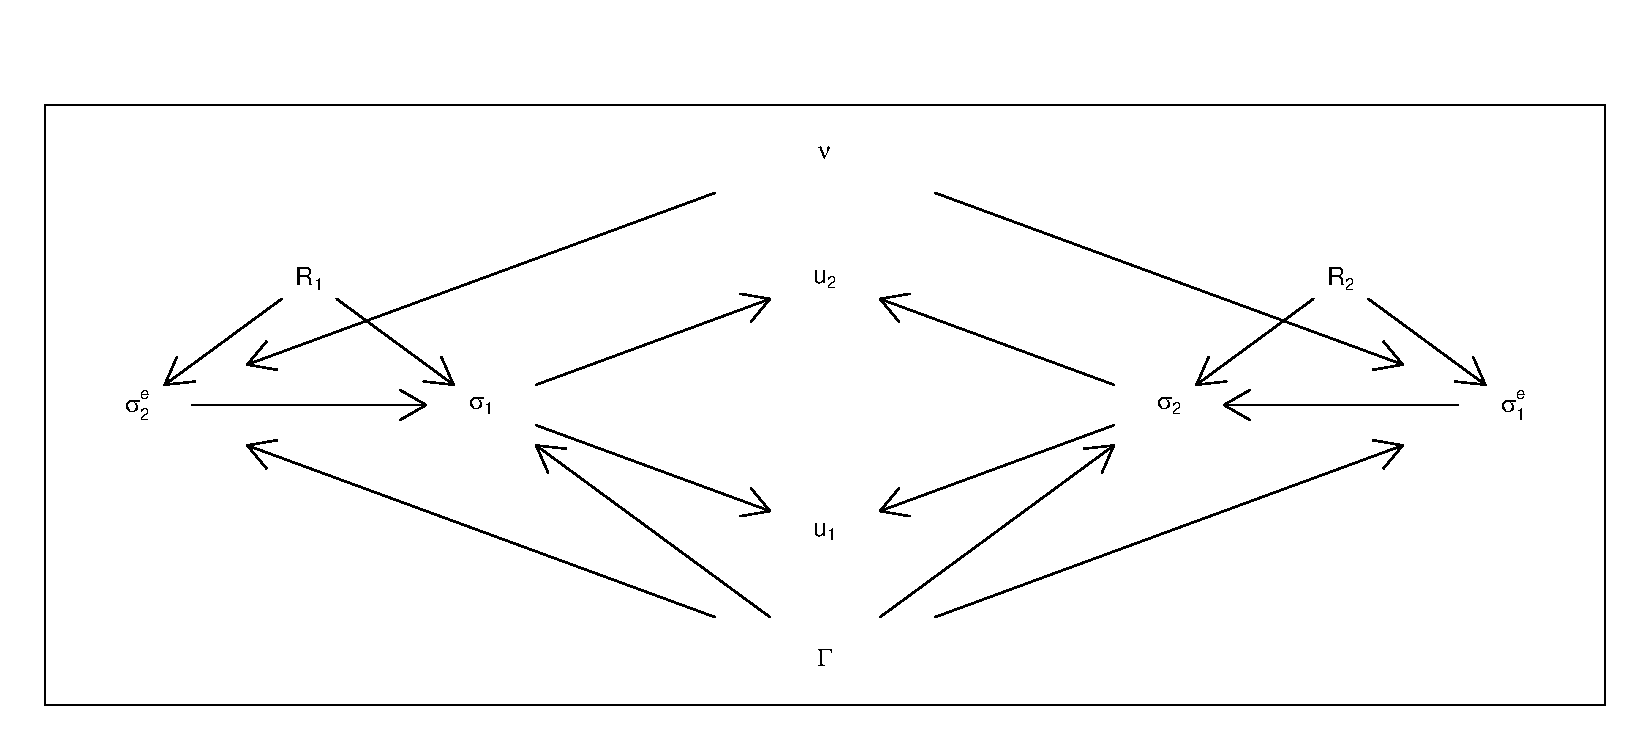
\includegraphics[width=0.8\linewidth]{ii_files/figure-latex/nfg5-1} 

}

\caption{A normal form game with a representation of equilibrium selection norms.}\label{fig:nfg5}
\end{figure}

We highlight three points from this discussion.

First the discussion highlights that thinking of theory as causal models does not force a sharp move away from abstract analytic theories; close analogues of these can often be incorporated in the same framework. This is true even for equilibrium analysis that seems to involve a kind of simultaneity on first blush.

Second, the discussion highlights how the causal modelling framework can make demands for specificity from formal theories. For instance specifying a functional relations from game form to actions requires a specification of a selection criterion in the event of multiple equilibria. Including agent rationality as a justification for the theory invites a specification for what would happen absent rationality.

Third the example shows a way of building a bridge from pure theory to empirical claims. One can think of Nash's theory as an entirely data free set of claims. When translated into an applied theory---a set of proposition about the ways actual players \emph{might} behave---and represented as a causal model, we are on a path to being able to use data to refine the theory. Thus we might begin with a formal specification like that in Figure \ref{fig:nfg5} but with initial uncertainty about player rationality, optimizing behavior, and equilibrium selection. This theory nests Nash but does not presume the theory to be a valid description of processes in the world. Combined with data, however, we shift to a more refined theory that selects Nash from the lower level model.

Finally, we can then apply the ideas of section \ref{theorygains} to applied formal theories and ask: is the theory useful? For instance, does data on player rationality help us better understand the relationship between game structure and welfare?

  \bibliography{bib.bib,packages.bib}

\end{document}
